%======================================================================
\section{System, model and ground truth}
\label{sec:system}
%======================================================================

%----------------------------------------------------------------------
\subsection{Two-dimensional Kuramoto--Sivashinsky}
\label{sec:ks2d}
%----------------------------------------------------------------------

The 2D experiments use the isotropic Kuramoto--Sivashinsky (KS) equation
\citep{kuramoto1976,sivashinsky1977,kalogirou2015},
\begin{equation}
  u_t + \nabla^2 u + \nabla^4 u + \tfrac12|\nabla u|^2 = 0,
  \qquad (x,y)\in[0,L)^2,
  \label{eq:ks2d}
\end{equation}
whose linear growth rate $K^2-K^4$ is positive on the ring $|\bm k|<1$ and
largest at $|\bm k|=1/\sqrt2$, which sets a pattern wavelength of
$2\sqrt2\,\pi\approx8.9$. Its nonlinearity drives the spatial mean of
$u$, which carries no dynamical information (only gradients of $u$ enter
the right-hand side), so we project the $\bm k=0$ mode out after every
step. The equation is integrated in Fourier space with a fourth-order
exponential time-differencing Runge--Kutta scheme (ETDRK4,
\citealp{kassam2005}) in double precision, with solver step $0.02$,
snapshot interval $\Delta t=0.1$ and grid spacing $\Delta x=0.344$
($128$ points at $L=44$). Figure~\ref{fig:systems} shows the domain whose
windows train the model.

The training data are four trajectories (plus one for validation) of 25
time units on a single periodic domain of side $264=6\times44$ ($768^2$
points), after a spin-up of 200 time units. The model is deployed on
square periodic domains of side $44$, $66$, $88$, $220$, $330$ and $440$, which
are all multiples of the site length $h=5.5$.

\para{Ground truth.} The Lyapunov spectrum of the PDE is computed with
the Benettin algorithm \citep{benettin1980} and the exact tangent
dynamics of the time-stepper, over 40-unit windows (about 7 Lyapunov
times) after a spin-up of 200 time units (protocol in
Appendix~\ref{app:groundtruth} and Paper~I). At $44^2$ three independent
runs give $\DKY=80.7$, $81.8$ and $83.6$ (mean $82.0$), with $42$--$44$ positive
exponents and $\lambda_1=0.165$--$0.194$; at $66^2$ two runs give $185.6$ and
$192.5$ (mean $189.0$), with $93$--$101$ positive exponents. The densities,
$0.0424$ and $0.0434$ per unit area, differ by $2.5\%$, inside the spread of
the individual runs, and the running estimates still move by $3$--$5\%$ over
the last 20 time units, so we treat the truths as uncertain at the level
of a few percent. Larger domains are beyond a full Lyapunov computation
(the expected dimension at $88^2$ is about 330); there the evidence that the
model remains faithful is the filter's own behaviour
(Sec.~\ref{sec:da_2d}) and the transfer results of Paper~I.

\begin{figure}[htbp]
\centering
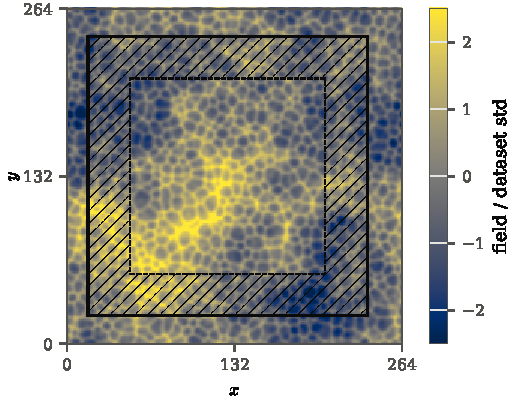
\includegraphics{figures/systems_ks2d.pdf}
\caption{One snapshot of 2D KS on the $264^2$ periodic domain whose
windows train the model, divided by the training standard deviation. The
outlined square is one $40\times40$-site training window, its forced halo
(six sites) hatched and its free interior inside the dashed line. Cells of
a fixed size fill the domain, which therefore holds many independent
copies of the local dynamics; this is what window training samples. The
training fields of the model used here additionally carry noise of
standard deviation $0.1$ (not shown).}
\label{fig:systems}
\end{figure}

%----------------------------------------------------------------------
\subsection{The model and its validation}
\label{sec:model_validation}
%----------------------------------------------------------------------

All 2D experiments use one model: the architecture and window training of
Paper~I with $c=12$ channels per site instead of 6, patches of $16\times16$
grid points ($h=5.5$), a propagator reach of $6$ sites, and the noisy
training of Sec.~\ref{sec:local_field} (settings in
Table~\ref{tab:architecture}). On a $44^2$ domain it has $64$ sites and
$\dlat=768$ latent coordinates; on $440^2$, $6400$ sites and $76\,800$, with the
same weights. We use 12 channels rather than the 6 of Paper~I because the
filter benefits from the extra capacity.

Table~\ref{tab:model_validation} compares the model with the truth.
Its Kaplan--Yorke dimension is $84.7$ at $44^2$ and $188.5$ at $66^2$, $3.6\%$ above
and $2.1\%$ below the truth run from the same initial condition; at $44^2$ it
lies just above the range of the three truth runs, at $66^2$ inside the
range of the two. Its number of positive exponents, $43$ and $94$, is inside
the truth's range at both sizes. Its leading exponent, $0.221$ and $0.217$, is
larger than the truth's ($0.165$--$0.194$ and $0.189$--$0.204$): errors grow
somewhat faster in the model than in the PDE. In free rollouts of 1000 steps
its field standard deviation is $5$--$7\%$ above the truth's from the same
initial conditions, and it carries slightly too much energy at the
smallest scales. A clean-trained model with the same recipe is as close to
the truth; Sec.~\ref{sec:da_noisy} compares the two as filters. Scored the
same way, the 6-channel model of Paper~I is within $1.7\%$ and $2.4\%$ at the
same two sizes (Paper~I reports $2.0\%$ and $0.6\%$ as means over initial
conditions against the mean truths).

\begin{table*}[htbp]
\caption{Validation of the 12-channel 2D KS models against the PDE. The
model's Kaplan--Yorke dimension, leading exponent $\lambda_1$ and number of
positive exponents $n_+$ are from one initial condition (seed 0); the error is
relative to the truth run from the same initial condition, and the truth
columns give the range over the independent truth runs (three at $44^2$, two
at $66^2$). Free rollout: field standard deviation (field units) and the share
of energy at $|\bm k|\ge1.4$ (\%), model / truth, from two initial conditions,
steps 100--1000 of 1000. Noisy-trained: the model of every experiment in
this paper.}
\label{tab:model_validation}
\widetabular{llccccccccc}{
Model & Size & $\DKY$ & Error & Truth $\DKY$ & $\lambda_1$ & Truth $\lambda_1$ & $n_+$ & Truth $n_+$ & Std & Small-scale energy \\
\hline
\tabinput{tables/model_validation}}
\end{table*}

%----------------------------------------------------------------------
\subsection{One-dimensional Kuramoto--Sivashinsky}
\label{sec:ks1d}
%----------------------------------------------------------------------

Section~\ref{sec:da_1d} uses the 1D equation,
$u_t + u u_x + u_{xx} + u_{xxxx} = 0$ on $[0,L)$, and the 1D model of
Paper~I, trained on whole periodic domains of length $L=100$ (grid spacing
$0.39$, snapshot interval $\Delta t=1.0$), with $16$ sites of length $6.25$,
$c=3$ channels, and an encoder and decoder that mix six neighbouring sites
($\Renc=\Rdec=6$). Its decoder is therefore not per-patch, and
Proposition~\ref{prop:blockdiag} does not apply; the 1D filters localize
the latent covariance instead (Appendix~\ref{app:da_filters}). Paper~I shows
that this model transfers to $L=200$ and $400$ with its $\DKY$ within about one
percent of the truth's. The truth has $\DKY=45.2$ and $26$--$27$ positive exponents
at $L=200$, and $\DKY=89.6$ and $51$ positive exponents at $L=400$, so the number of
unstable directions doubles with the domain.
